\documentclass{article}
\usepackage{hyperref}
\usepackage{listings}
\usepackage{color}
\usepackage{xcolor}
\usepackage{geometry}
\usepackage{graphicx}
\usepackage{amsmath}
\usepackage{caption}
\usepackage{subcaption}
\usepackage{syntax}
\geometry{margin=1in}
\pdfminorversion=6

\newcommand\TODO[1]{\textcolor{red}{TODO: #1}}

\newcommand\header[2]{
    \begin{center}
        {\large
        UCSD CSE 291 (Differentiable Programming) Assignment #1: \\
        \vspace{0.3cm}
        \Large
        #2}
    \end{center}
}

\definecolor{dkgreen}{rgb}{0,0.6,0}
\definecolor{gray}{rgb}{0.5,0.5,0.5}
\definecolor{mauve}{rgb}{0.58,0,0.82}
\lstset{frame=tb,
        aboveskip=3mm,
        belowskip=3mm,
        showstringspaces=false,
        columns=flexible,
        basicstyle={\small\ttfamily},
        numbers=none,
        numberstyle=\tiny\color{gray},
        keywordstyle=\color{blue},
        commentstyle=\color{dkgreen},
        stringstyle=\color{mauve},
        breaklines=true,
        breakatwhitespace=true,
        tabsize=2
}

\hypersetup{colorlinks=true}


\begin{document}

\header{2}{Reverse mode automatic differentiation}

\section{Getting gradients by running the function backwards.}

In the second homework, we will implement what's called the reverse-mode automatic differentiation on straight-line code. It is equivalent (or can be seen as a generalization) of the popular backpropagation algorithm in deep learning. Before we talk about reverse mode, let's talk about why we need something other than the forward mode we implemented last time.

Consider a function $f(\mathbf{x})$ that takes many numbers and outputs a scalar $f(\mathbf{x}): \mathbb{R}^n \rightarrow \mathbb{R}$, where $n$ can be a large number (say, a million). Suppose we want to compute the gradient of $f$ (say, for optimizing or sampling $f$ using gradient-based methods). Applying forward mode differentiation to $f$ would give as a function $Df(\mathbf{x}, \mathbf{dx}) : \mathbb{R}^n \times \mathbb{R}^n \rightarrow \mathbb{R} \times \mathbb{R}$. Since $Df$ can only output one derivative at a time, we need to feed in $n$ different ``one-hot'' $\mathbf{dx}$ (where one component is $1$ and all others are $0$) in order to get the full gradient vector -- this is too inefficient. Instead, reverse mode gives us a function $D^{T}f(\mathbf{x}, dy) : \mathbb{R}^n \times \mathbb{R} \rightarrow \mathbb{R}^n$ that can give us the full gradient vector at once if we set $dy=1$.

How is this possible? Let's use the same example we used for forward mode:
\begin{lstlisting}[language=Python]
def f(x : In[float], y : In[float]) -> float:
	z0 : float = h(x, y)
	z1 : float = g(z0)
	return z1
\end{lstlisting}
Recall that the forward mode transform turns the function into their ``Df'' version.
\begin{lstlisting}[language=Python]
class _dfloat:
	val : float
	dval : float

def Df(x : In[_dfloat], y : In[_dfloat]) -> _dfloat:
	z0 : _dfloat = Dh(x, y)
	z1 : _dfloat = Dg(z0)
	return z1
\end{lstlisting}
In reverse mode, we want to turn \lstinline{f} into its \lstinline{DTf} version. The function signature of \lstinline{DTf} is:
\begin{lstlisting}[language=Python]
def DTf(x : In[float], _dx : Out[float], y : In[float], _dy : Out[float], dz1 : In[float])
\end{lstlisting}
It allows us to input \lstinline{x}, \lstinline{y}, and \lstinline{dz1} (usually called the ``adjoint''), and receive the derivatives $dz_1 \cdot \frac{\partial f}{\partial x}$ and $dz_1 \cdot \frac{\partial f}{\partial y}$ in \lstinline{_dx} and \lstinline{_dy}.

Suppose we also have \lstinline{DTh} and \lstinline{DTg}:
\begin{lstlisting}[language=Python]
def DTh(x : In[float], _dx : Out[float], y : In[float], _dy : Out[float], dz0 : In[float])
def DTg(z0 : In[float], _dz0 : Out[float], dz1 : In[float])
\end{lstlisting}
How do we use them to assemble our target \lstinline{DTf}?

Notice that the input of \lstinline{DTg} requires the adjoint \lstinline{dz1} from the input of \lstinline{DTf}, and the input of \lstinline{DTh} requires the adjoint \lstinline{dz0} from the output of \lstinline{DTg} (through \lstinline{_dz0}). Thus, the only sensible way to properly assemble these functions is the following:
\begin{lstlisting}[language=Python]
def DTf(x : In[float], _dx : Out[float], y : In[float], _dy : Out[float], dz1 : In[float]):
	# First, run the function forward
	z0 : float = h(x, y)
	z1 : float = g(z0)
	# Next, run it backwards
	_dz0 : float
	DTg(z0, _dz0, dz1) # output _dz0
	DTh(x, _dx, y, _dy, _dz0) # DTh will write the outputs in x and y 
\end{lstlisting}
Suppose \lstinline{DTh} and \lstinline{DTg} takes around the same time as \lstinline{h} and \lstinline{g}, respectively, then \lstinline{DTf} would take around two times to compute as \lstinline{f} -- we can compute the gradients cheaply regardless of the number of input variables! (This argument breaks when we have recursive functions or simply have very deeply nested function call, in the homework we ignore this, but we will discuss this in much more details in the class).

Like in the forward mode, we need the list of ``terminal'' cases:
\begin{equation}
\begin{aligned}
\text{DTConstant}(c, dz) &= \left[dc \leftarrow 0\right] \\
\text{DTVariable}(x, dz) &= \left[dx += dz\right] \\
\text{DTAdd}(x, y, dz) &= \left[dx += dz, dy += dz\right] \\
\text{DTSub}(x, y, dz) &= \left[dx += dz, dy += -dz\right] \\
\text{DTMul}(x, y, dz) &= \left[dx += dz \cdot y, dy += dz \cdot x\right] \\
\text{DTDiv}(x, y, dz) &= \left[dx += \frac{dz}{y}, dy += \frac{-dz \cdot x}{y^2}\right] \\
\text{DTSin}(x, dz) &= \left(dx += dz \cdot \cos(x)\right) \\
\text{DTCos}(x, dz) &= \left(dx += -dz \cdot \sin(x)\right) \\
\text{DSqrt}(x, dz) &= \left(dx += \frac{dz}{2\sqrt{x}} \right) \\
\text{DPow}(x, y, dz) &= \left(dx += dz \cdot y \cdot x^{y-1}, dy += dz \cdot x^y \log(x) \right) \\
\text{DExp}(x, dz) &= \left(dx += dz \cdot \exp(x) \right) \\
\text{DLog}(x, dz) &= \left(dx += \frac{dz}{x} \right) \\
\text{Dfloat2int}(x, dz) &= \left(dx += 0\right)
\end{aligned}
\end{equation}

\section{Reverse-mode automatic differentiation in loma}

Just like the forward mode differentiation, the reverse mode can be defined as the following in loma:
\begin{lstlisting}[language=Python]
def f(x : float) -> float:
	# ...

df = rev_diff(f) # df has type In[float], Out[float] -> void
\end{lstlisting}

The transformation will happen in \lstinline{autodiff.py} and \lstinline{reverse_diff.py}. \textbf{Your task is to fill in the blanks in the \lstinline{reverse_diff} function in \lstinline{reverse_diff.py}. Use \lstinline{hw_tests/hw2/test.py} to test your implementation. If you pass all tests, you get full points. Each test is weighted equally.}

\subsection{Function type after reverse mode transformation.}
\label{sec:reversemodespec}

Given a function \lstinline{f(x0 : In[T0], x1 : Out[T1], ...) -> T}, reverse mode will transform the signature to \lstinline{DTf(x0 : In[T0], _dx0 : Out[T0], x1 : In[T1], ..., _dout : In[T])}. For an input argument \lstinline{x}, there are two cases:
\begin{itemize}
	\item \lstinline{x : In[T]} is only used as an input. We will append the adjoint output \lstinline{_dx : Out[T]} right after \lstinline{x}. Importantly, we will add the derivatives to the existing differential in \lstinline{_dx}, instead of overwriting it. This eliminates the need to initialize the data structure to zero, which can be costly in some cases.
	\item \lstinline{x : Out[T]} is only used as an output. We transform the argument to an adjoint input \lstinline{x : In[T]]}. The original output argument is removed.
\end{itemize}

\paragraph{Handling argument name collision.} We need to generate several new arguments for our reverse mode transform. It is possible that the name of these new argument collide with existing arguments. This can cause problems when we want to do nested differentiation in the next homework. My (hacky) solution is to append a random string for each generated argument. For example, the following function:
\begin{lstlisting}[language=Python]
def foo(x : In[float], y : Out[float]) -> float:
    # ...

d_foo = rev_diff(foo)
\end{lstlisting}
would be transformed into
\begin{lstlisting}[language=Python]
def foo(x : In[float], _dx_Ibx3EY : Out[float], y : In[float], _dreturn_W7TFYQ : In[float]):
    # ...

d_foo = rev_diff(foo)
\end{lstlisting}
and we hope that the random strings do not collide with each other by chance. You can use the \lstinline{random_id_generator} in \lstinline{reverse_diff.py} (which I stole from some \href{https://stackoverflow.com/questions/2257441/random-string-generation-with-upper-case-letters-and-digits}{nice Stackoverflow post}) to achieve this. You do not have to do this in this homework, but you will need to have something like this for the nested differentiation in the next homework.

In the reference code below, I remove the random string for better readability.

\subsection{Transformation of statements and expressions}
As in the previous homework, we will implement an \lstinline{IRMutator} to transform the code to its reverse-mode derivatives. As usual, we recommend you to try to pass the tests one-by-one. 

\paragraph{test_identity} The task again asks you to transform the following identity function:
\begin{lstlisting}[language=Python]
def identity(x : In[float]) -> float:
    return x

d_identity = rev_diff(identity)
\end{lstlisting}
The reverse mode transformation should give the equivalent of the following function:
\begin{lstlisting}[language=Python]
def d_identity(x : In[float], _dx : Out[float], _dreturn : In[float]):
	_dx = _dx + _dreturn
\end{lstlisting}
(Compare the result to the forward mode transformation -- how is it different?)

You will need to implement \lstinline{mutate_function_def}, \lstinline{mutate_return}, and \lstinline{mutate_var} for the transformation. For \lstinline{mutate_function_def}, you need to come up with the new argument types of \lstinline{d_identity}. Next, you need to visit the statement in reverse order to accumulate the derivatives. For \lstinline{mutate_var}, I recommend returning a Python \lstinline{list} that contains a statement for the adjoint accumulation. Something like 
\begin{lstlisting}[language=Python]
return [loma_ir.Assign(loma_ir.Var('_dx'), loma_ir.BinaryOp(loma_ir.Add(), loma_ir.Var('_dx'), loma_ir.Var('_dreturn')))]
\end{lstlisting}
I used a class variable \lstinline{self.adjoint} to pass around the adjoint from the return statement.
Finally, for \lstinline{mutate_return}, you want to setup the adjoint \lstinline{self.adjoint}, and get the accumulation statements from the expression and return them.

\paragraph{test_constant} This one should be easy: given the following constant function
\begin{lstlisting}[language=Python]
def constant(x : In[float]) -> float:
    return 2.0

d_constant = rev_diff(constant)
\end{lstlisting}
You should turn it to a ``no-op'' function:
\begin{lstlisting}[language=Python]
def d_constant(x : In[float], _dx : Out[float], _dreturn : In[float]):
	pass
\end{lstlisting}
You will need to implement \lstinline{mutate_const_float} to pass this test.

\paragraph{test_plus, test_subtract, test_multiply, and test_divide} These tests ask you to transform the following binary operations:
\begin{lstlisting}[language=Python]
def plus(x : float, y : float) -> float:
    return x + y

d_plus = rev_diff(plus)

def subtract(x : float, y : float) -> float:
    return x - y

d_subtract = rev_diff(subtract)

def multiply(x : float, y : float) -> float:
    return x * y

d_multiply = rev_diff(multiply)

def divide(x : float, y : float) -> float:
    return x / y

d_divide = rev_diff(divide)
\end{lstlisting}

You'll need to implement \lstinline{mutate_add}, \lstinline{mutate_sub}, \lstinline{mutate_mul}, and \lstinline{mutate_div}. Like \lstinline{mutate_var}, I recommend you implement it so that each of them returns a list of adjoint accumulation statements. For example, \lstinline{mutate_add} should pass the adjoint from the parent expression to the two children, and return all the adjoint accumulation statements it gets from the children.

We provide our output for \lstinline{d_plus} as an example:
\begin{lstlisting}[language=Python]
def d_plus(x : In[float], _dx : Out[float], y : In[float], _dy : Out[float], _dreturn : In[float]):
	_dx = _dx + _dreturn;
	_dy = _dy + _dreturn;
\end{lstlisting}

\paragraph{test_square} This one tests if you handle multiple use of one variable inside an expression correctly:
\begin{lstlisting}[language=Python]
def square(x : In[float]) -> float:
    return x * x

d_square = rev_diff(square)
\end{lstlisting}
Our output is
\begin{lstlisting}[language=Python]
def d_square(x : In[float], _dx : Out[float], _dreturn : In[float]):
	_dx = _dx + x * _dreturn + x * _dreturn;
\end{lstlisting}

\paragraph{test_declare} Things will get a bit more complicated from now on. The test asks you to transform the following sequence of variable declarations:
\begin{lstlisting}[language=Python]
def declare(x : In[float], y : In[float]) -> float:
    z0 : float = x + y
    z1 : float = z0 + 5.0
    z2 : float = z1 * z0
    z3 : float = z2 / z1
    z4 : float = z3 - x
    return z4

d_declare = rev_diff(declare)
\end{lstlisting}
The reverse mode transformation should gives the following code:
\begin{lstlisting}[language=Python]
def d_declare(x : In[float], _dx : Out[float], y : In[float], _dy : Out[float], _dreturn : In[float]):
	# Forward pass: execute the primal code
	z0 : float = x + y
	_dz0 : float # automatically initialized to zero
	z1 : float = z0 + 5.0
	_dz1 : float
	z2 : float = z1 * z0
	_dz2 : float
	z3 : float = z2.val / z1.val
	_dz3 : float
	z4 : float = z3.val - x.val
	_dz4 : float
	# Reverse pass: traverse the code backwards
	_dz4 = _dz4 + _dreturn
	_dz3 = _dz3 + _dz4
	_dx = _dx + (0.0 - _dz4)
	_dz2 = _dz2 + _dz3 / z1
	_dz1 = _dz1 + (0.0 - _dz3 * z2 / z1 * z1)
	_dz1 = _dz1 + z0 * _dz2
	_dz0 = _dz0 + z1 * _dz2
	_dz0 = _dz0 + _dz1
	_dx = _dx + _dz0
	_dy = _dy + _dz0
\end{lstlisting}

The transformation would first take the primal (original) code and append a differential (say, \lstinline{_dz0}) initialized to zero after each declaration. The primal values (say, \lstinline{z2}) can be used later in the reverse pass. The differentials will later be used for storing the derivatives. Next, we run the statements backwards (from \lstinline{z4} to \lstinline{z0}), and accumulate the derivatives like before.

You should first modify \lstinline{mutate_function_def} to add the forward pass generation. I implemented this by adding another \lstinline{IRMutator} for transforming the primal function. Next, you should implement \lstinline{mutate_declare} in \lstinline{RevDiffMutator} to backpropagate the derivatives.

\paragraph{test_assign1-5 and test_assign_args} The assign statements are trickier to handle since they may overwrite the values we want to reuse later in the reverse pass. Our solution is to cache the overwritten values into an array, so that we can reuse it later. For example, in \lstinline{test_assign2}, we are asked to differentiate the following function:
\begin{lstlisting}[language=Python]
def assign2(x : In[float], y : In[float]) -> float:
    z : float
    z = 2.5 * x - 3.0 * y
    z = z + x * y
    return z

d_assign2 = rev_diff(assign2)
\end{lstlisting}

My implementation would generate the following code:
\begin{lstlisting}[language=Python]
def d_assign2(x : In[float], _dx : Out[float], y : In[float], _dy : Out[float], _dreturn : In[float]):
	# Forward pass
	_t_float : Array[float, 2]
	_stack_ptr_float : int
	z : float
	_dz_ : float
	# cache z's value in a stack _t_float before it's overwritten
	_t_float[_stack_ptr_float] = z
	_stack_ptr_float = _stack_ptr_float + 1 # advance pointer
	z = 2.5 * x - 3.0 * y
	# cache z's value in a stack _t_float before it's overwritten
	_t_float[_stack_ptr_float] = z
	_stack_ptr_float = _stack_ptr_float + 1 # advance pointer
	z = z + x * y
	# Reverse pass
	_adj_0 : float # some tmp variables for later use
	_adj_1 : float
	_adj_2 : float
	_adj_3 : float
	_adj_4 : float
	# Backprop "return z"
	_dz_ = _dz_ + _dreturn_
	# Backprop "z = z + x * y"
	# First, recover the value of z before overwrite
	# by poping the value from the stack "_t_float"
	_stack_ptr_float = _stack_ptr_float - 1
	z = _t_float[_stack_ptr_float]
	# Next, compute the adjoints of the three inputs:
	# z, x, and y and store them into _adj_0, _adj_1, and _adj_2
	_adj_0 = _dz_
	_adj_1 = y * _dz_
	_adj_2 = x * _dz_
	# Zero the differential of z to account for the effect of
	# overwrite
	_dz_ = 0.0
	# Accumulate the adjoints _adj_0, _adj_1, and _adj_2
	# to z, x, y's differentials respectively
	_dz_ = (_dz_) + (_adj_0);
	(*_dx_) = ((*_dx_)) + (_adj_1);
	(*_dy_) = ((*_dy_)) + (_adj_2);
	# Backprop "z = 2.5 * x - 3.0 * y"
	# Recover the value of z from the stack
	_stack_ptr_float = (_stack_ptr_float) - ((int)(1));
	z = (_t_float)[_stack_ptr_float];
	# Compute the adjoints and store them into
	# temporary variables
	_adj_3 = ((float)(2.5)) * (_dz_);
	_adj_4 = ((float)(3.0)) * (((float)(0.0)) - (_dz_));
	# Zero the differential of z
	_dz_ = (float)(0.0);
	# Accumulate the adjoints
	(*_dx_) = ((*_dx_)) + (_adj_3);
	(*_dy_) = ((*_dy_)) + (_adj_4);
\end{lstlisting}

The generated code is a bit involved. Let's look at them line by line. Firstly, in the forward pass, we
first allocate an array \lstinline{_t_float}, acting as a stack for storing the values from forward pass (line 3). We also declare a ``pointer'' integer to indicate the current writing position (line 4). Before each assign statement, we cache the left hand side values to the array, so that we don't lose the values (line 8-9 and 12-13).

In the reverse pass, for each assign statement \lstinline{z = f(x0, x1, ... z)}, we need to to the following:
\begin{enumerate}
	\item First, pop from the cache: \lstinline{z = stack.pop()} (line 26-27 and 43-44).
	\item Next, store the adjoints for all the inputs to \lstinline{f}: \lstinline{_adj_x0 = ...}, \lstinline{_adj_x1 = ...}, and \lstinline{_adj_z = ...}. (line 30-32 and line 47-48).
	\item Next, zero the differential of z: \lstinline{_dz = 0} (line 35 and 50).
	\item Next, accumulate the adjoint variables to their corresponding differentials: \lstinline{_dx0 += _adj_x0}, \lstinline{_dx1 += _adj_x1}, ... \lstinline{_dz += _adj_z}. (line 38-40 and 52-53)
\end{enumerate}
(Think: what happens if we don't first store the adjoints in these temporary variables, and directly accumulate them to the target differentials?)

You'll need to modify \lstinline{mutate_function_def} and add implementation to \lstinline{mutate_assign} to pass these tests.

To come up with the name of the temporary arrays, I found the following utility function to be useful to turn the type's name into a string:
\begin{lstlisting}[language=Python]
def type_to_string(t):
    match t:
        case loma_ir.Int():
            return 'int'
        case loma_ir.Float():
            return 'float'
        case loma_ir.Array():
            return 'array_' + type_to_string(t.t)
        case loma_ir.Struct():
            return t.id
        case _:
            assert False
\end{lstlisting}
You can find it in \lstinline{reverse_diff.py}.

\paragraph{test_refs_out} This test checks if you handles an output argument correctly. If the left hand side of an assign statement is an output argument in the primal function, you should ignore it in the forward pass (since we don't have an output argument to write to). I used the following function to determine if the left hand side of an assign statement is part of the output arguments:
\begin{lstlisting}[language=Python]
def check_lhs_is_output_arg(lhs, output_args):
    match lhs:
        case loma_ir.Var():
            return lhs.id in output_args
        case loma_ir.StructAccess():
            return check_lhs_is_output_arg(lhs.struct, output_args)
        case loma_ir.ArrayAccess():
            return check_lhs_is_output_arg(lhs.array, output_args)
        case _:
            assert False
\end{lstlisting}
Here, \lstinline{output_args} is a Python \lstinline{set} that contains a list of strings that are the output arguments of the function.

\paragraph{test_call_sin, test_call_cos, test_call_sqrt, test_call_pow, test_call_exp, test_call_log, test_call} You'll implement \lstinline{mutate_call} to handle these tests. They should not be that different from the binary operations.

\paragraph{test_int_input, test_int_output, test_int_assign} These test whether your code can handle integer variables. You should properly ignore adjoints for integers in your generated code. Assignment to an integer variable requires a bit of special handling: recall that we use an array to cache the values that are overwritten. We now need two arrays: one for floats and one for integers.

\paragraph{test_array_output, test_array_input, test_int_array_input, test_array_input_indexing, test_array_output_indexing, test_sum_nested_array} These test your handling of array expressions. Arrays shouldn't be that different from other expressions. Make sure you handle the case when there is an array access on the left hand side of an assign statement: you want to backpropagate correctly to the right index.

\paragraph{test_struct_input, test_nested_struct_input, test_struct_output, test_struct_declare, test_struct_assign} These test whether you handle structs correctly. Structs require a little bit more massages to code generation. Firstly, you will need a way to assign zero to a struct (for the assign statement). I use the following function:
\begin{lstlisting}[language=Python]
def assign_zero(target):
    match target.t:
        case loma_ir.Int():
            return []
        case loma_ir.Float():
            return [loma_ir.Assign(target, loma_ir.ConstFloat(0.0))]
        case loma_ir.Struct():
            s = target.t
            stmts = []
            for m in s.members:
                target_m = loma_ir.StructAccess(
                    target, m.id, t = m.t)
                if isinstance(m.t, loma_ir.Float):
                    stmts += assign_zero(target_m)
                elif isinstance(m.t, loma_ir.Int):
                    pass
                elif isinstance(m.t, loma_ir.Struct):
                    stmts += assign_zero(target_m)
                else:
                    assert isinstance(m.t, loma_ir.Array)
                    assert m.t.static_size is not None
                    for i in range(m.t.static_size):
                        target_m = loma_ir.ArrayAccess(
                            target_m, loma_ir.ConstInt(i), t = m.t.t)
                        stmts += assign_zero(target_m)
            return stmts
        case _:
            assert False
\end{lstlisting}
Next, you need a way to accumulate derivatives to a struct. I use the following function:
\begin{lstlisting}[language=Python]
def accum_deriv(target, deriv, overwrite):
    match target.t:
        case loma_ir.Int():
            return []
        case loma_ir.Float():
            if overwrite:
                return [loma_ir.Assign(target, deriv)]
            else:
                return [loma_ir.Assign(target,
                    loma_ir.BinaryOp(loma_ir.Add(), target, deriv))]
        case loma_ir.Struct():
            s = target.t
            stmts = []
            for m in s.members:
                target_m = loma_ir.StructAccess(
                    target, m.id, t = m.t)
                deriv_m = loma_ir.StructAccess(
                    deriv, m.id, t = m.t)
                if isinstance(m.t, loma_ir.Float):
                    stmts += accum_deriv(target_m, deriv_m, overwrite)
                elif isinstance(m.t, loma_ir.Int):
                    pass
                elif isinstance(m.t, loma_ir.Struct):
                    stmts += accum_deriv(target_m, deriv_m, overwrite)
                else:
                    assert isinstance(m.t, loma_ir.Array)
                    assert m.t.static_size is not None
                    for i in range(m.t.static_size):
                        target_m = loma_ir.ArrayAccess(
                            target_m, loma_ir.ConstInt(i), t = m.t.t)
                        deriv_m = loma_ir.ArrayAccess(
                            deriv_m, loma_ir.ConstInt(i), t = m.t.t)
                        stmts += accum_deriv(target_m, deriv_m, overwrite)
            return stmts
        case _:
            assert False
\end{lstlisting}
If \lstinline{overwrite} argument is true, \lstinline{accum_deriv} would just overwrite the derivatives (this is for things like the \lstinline{_adj} temporary variables we create during the handling of assign statements). Otherwise it accumulates on the existing derivatives. 

\paragraph{test_multivariate} This test demonstrates how reverse mode would usually be used in loma code:
\begin{lstlisting}[language=Python]
def multivariate(x : In[float], y : In[float]) -> float:
    return 3 * x * cos(y) + y * y

d_multivariate = rev_diff(multivariate)

def multivariate_grad(x : In[float], y : In[float], dx : Out[float], dy : Out[float]):
    d_multivariate(x, dx, y, dy, 1.0)
\end{lstlisting}
You probably don't need to implement anything extra to pass this test.

\section{Reverse mode in action}
Now we actually put reverse mode into use. Like the previous homework, you don't have to write any code here and this part is not graded. You can run the code and see some optimization in action. 

\begin{figure}
\centering
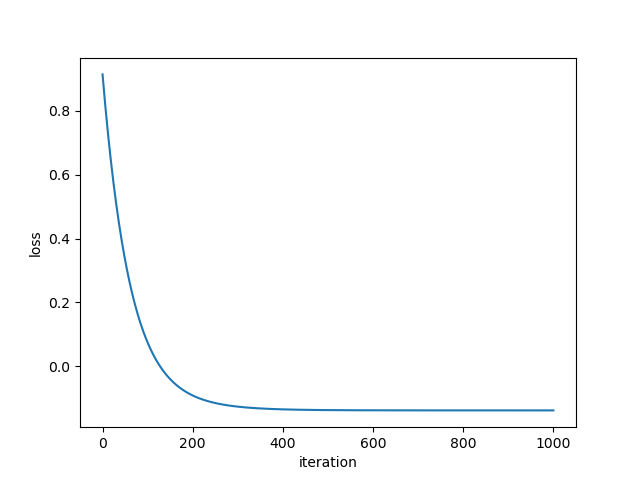
\includegraphics[width=0.8\linewidth]{imgs/loss-bigger-poly.png}
\caption{Loss curve of the gradient descent process for \lstinline{bigger_poly}.}
\label{fig:optimize}
\end{figure}

\paragraph{Optimizing a bigger polynomial function.} \lstinline{optimize_poly_rev} does similar thing as \lstinline{optimize_poly_fwd}, but it takes an array of size 5 instead of just two variables as input. Since it's hard to visualize the 5D trajectory, we show how the loss decreases in Figure~\ref{fig:optimize}.

\paragraph{Mass spring system.} Let's implement a mass spring system using Hamiltonian mechanics. Remember our Hamiltonian system looks like this:
\begin{equation}
\begin{aligned}
\dot{\mathbf{q}} &= \frac{\partial}{\partial \mathbf{p}} H(\mathbf{q}, \mathbf{p}) \\
\dot{\mathbf{p}} &= -\frac{\partial}{\partial \mathbf{q}} H(\mathbf{q}, \mathbf{p})
\end{aligned}.
\end{equation}

This time, the state $\mathbf{q}$ is the 2D positions of some mass spring nodes (so $\mathbf{q} \in \mathbb{R}^{2n}$ where $n$ is the number of nodes). Reminder that the Hamiltonian $H$ is composed of kinetic energy $K$ and potential energy $U$:
\begin{equation}
H = K + U
\end{equation}

The kinetic energy is straightforward this time since we're not using generalized coordinates ($\mathbf{p}$ is the usual momentum $m \dot{q}$):
\begin{equation}
K = \sum_{i=0}^{2n} \frac{1}{2} \frac{p_i^2}{m}
\end{equation}
where $m$ is the mass.

The potential energy is the mass spring energy plus the gravity:
\begin{equation}
U = \sum_{i=0}^{n-1} \frac{1}{2} k \left(\sqrt{\left(q_{2i} - q_{2i + 2}\right)^2 + \left(q_{2i+1} - q_{2i+3}\right)^2} - l\right)^2 + \sum_{i=0}^{n} m g q_{2i+1},
\end{equation}
where $k$ is the Hooke's law constant (the larger the more ``bouncy'' the mass spring becomes), $l$ is the length of the mass spring, and $g$ is the gravitational constant. The weird indexing is there to extract the x and y coordinates.

The following loma code implements the Hamiltonian energy (see \lstinline{examples/mass_spring_rev.py}):
\begin{lstlisting}[language=Python]
class MassSpringConfig:
    mass : float
    length : float
    k : float
    g : float

def hamiltonian(q : In[Array[float]], p : In[Array[float]], c : In[MassSpringConfig]) -> float:
    K : float
    K = K + 0.5 * p[0] * p[0] / c.mass
    K = K + 0.5 * p[1] * p[1] / c.mass
    K = K + 0.5 * p[2] * p[2] / c.mass
    K = K + 0.5 * p[3] * p[3] / c.mass
    K = K + 0.5 * p[4] * p[4] / c.mass
    K = K + 0.5 * p[5] * p[5] / c.mass
    K = K + 0.5 * p[6] * p[6] / c.mass
    K = K + 0.5 * p[7] * p[7] / c.mass
    K = K + 0.5 * p[8] * p[8] / c.mass
    K = K + 0.5 * p[9] * p[9] / c.mass

    U : float
    # mass spring potential
    tmp : float = sqrt((q[0] - q[2]) * (q[0] - q[2]) + (q[1] - q[3]) * (q[1] - q[3])) - c.length
    U = U + 0.5 * c.k * tmp * tmp
    tmp = sqrt((q[2] - q[4]) * (q[2] - q[4]) + (q[3] - q[5]) * (q[3] - q[5])) - c.length
    U = U + 0.5 * c.k * tmp * tmp
    tmp = sqrt((q[4] - q[6]) * (q[4] - q[6]) + (q[5] - q[7]) * (q[5] - q[7])) - c.length
    U = U + 0.5 * c.k * tmp * tmp
    tmp = sqrt((q[6] - q[8]) * (q[6] - q[8]) + (q[7] - q[9]) * (q[7] - q[9])) - c.length
    U = U + 0.5 * c.k * tmp * tmp
    # gravity potential
    U = U + c.mass * c.g * q[1]
    U = U + c.mass * c.g * q[3]
    U = U + c.mass * c.g * q[5]
    U = U + c.mass * c.g * q[7]
    U = U + c.mass * c.g * q[9]

    return K + U

d_hamiltonian = rev_diff(hamiltonian)

def gradH(q : In[Array[float]], p : In[Array[float]], c : In[MassSpringConfig],
          dq : Out[Array[float]], dp : Out[Array[float]]):
    d_c : MassSpringConfig
    d_hamiltonian(q, dq, p, dp, c, d_c, 1.0)
\end{lstlisting}

To make the animation more interesting, we added two things outside of loma: we fix the position and momentum of the first mass spring node, and we added an exponential ``damping'' factor that reduces the momentum at each frame.

See \lstinline{examples/mass_spring_rev.mp4} for the generated animation.

\end{document}
